% Este arquivo tex vai ser incluído no arquivo tex principal, não pe preciso
% declarar nenhum cabeçalho

\section{Comida}
\subsection{Bandejão}

Um dos momentos de glória do dia de um futuro engenheiro, cientista ou bacharel
é o Bandejão. É a hora de intensas e indiscutíveis emoções. Caso sua salada
corra sobre a mesa, mantenha-se calmo. Evite discussões, jamais tente descobrir
o sabor do suco pelo paladar (caju ou manga?). É mais cômodo ler no cardápio do
dia. Uma dica: para cortar o bife faça muita força e, quando começar a amolecer,
pare, você chegou na bandeja.

Falando sério agora: o Bandejão (Restaurante Universitário), Bandex ou Bandeco
fica ao lado da Biblioteca Central, bem em frente ao PB (Prédio Básico, ou Ciclo
Básico II) e, a menos que você não queira economizar uma boa grana com comida,
vai ser o lugar onde você vai estar na maioria dos seus horários de almoço. Com
o tempo, você vai ver que o Bandeco é o ``coração da Unicamp''. É o local de
você se encontrar com os amigos (combinando ou não antes), contar os micos nas
aulas, jogar conversa fora e falar mal da comida, que nem é tão ruim assim como
muitos dizem. Sem dúvida, é o melhor custo-benefício da Unicamp. Por R\$2,00,
você tem direito a arroz, feijão, salada, proteína de soja, suco, chá e café à
vontade.  A carne e a sobremesa tem que dar uma choradinha para a tiazinha para
poder repetir, mas geralmente dá certo.

\begin{figure}[h!]
    \centering
    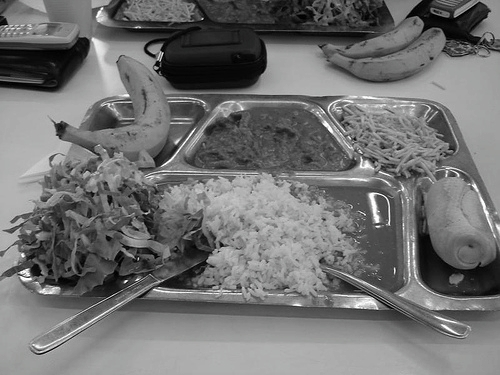
\includegraphics[width=.45\textwidth]{img/barao/bandeco.jpg}
\end{figure}

Existe também o RA (Restaurante Administrativo), também conhecido como Pratex,
pelo fato de a comida ser servida em pratos e não em bandejas. Fica atrás da
Faculdade de Engenharia Elétrica e de Computação (FEEC), perto do prédio da
Engenharia Básica. Tem algumas diferenças em relação ao Bandex: o espaço físico
é bem menor, por exemplo. No RA você mesmo se serve, apesar de a carne às vezes
ser servida pela tia que trabalha lá. Se você for com um amigo, vá com paciência
para esperar, porque é difícil para arrumar lugar, além ser apertado. Dependendo
de onde você vai ter aula antes ou depois do almoço, é mais negócio almoçar no
RA. Para poder usar o Bandex e o RA, você deve estar com o seu Cartão
Universitário (CU) carregado.

Além do RA, há o novo restaurante universitário, conhecido como RS (Restaurante
Universitário da Saturnino). Ele é localizado próximo ao IC-3 e ao prédio azul
da Civil. Semelhante ao RA, você come em pratos, as tias servem a carne e o
resto é self-service. As vantagens são que o ambiente é menos claustrofóbico, há
mais lugares e a localização o torna muito prático para os computeiros. Porém,
só está aberto no período do almoço, e não há como carregar o cartão por lá.

\subsubsection*{Como funciona o esquema de carregar o cartão?}

Simples. Você vai ao guichê ao lado direito da entrada do Bandex e faz, por
exemplo, um depósito de R\$20,00 para 10 créditos. Outra maneira de colocar
créditos no CU é fazer um depósito na conta do Bandex no Santander (Ag.: 207 /
Conta: 43.010.009-2) ou no Banco do Brasil (Ag.: 4203-X / Conta: 66.315-8) e
depois carregar o seu cartão, no guichê do Bandex ou na Prefeitura do Campus
(próximo à Reitoria), apresentando o comprovante de depósito. Não são aceitos
comprovantes de pagamento de entrega de envelope ou via internet. Fique esperto
para não ir ao RA ou RS sem créditos, porque lá não dá pra carregar o cartão e
você terá que andar até o Bandeco.

Os restaurantes funcionam de segunda a sexta, nos seguintes horários:

\begin{itemize}
    \item  RU, das 10h30 às 14h (almoço) e das 17h30 às 19h45 (jantar).
    \item  RA, das 11h30 às 14h (almoço) e das 17h30 às 19h (jantar).
    \item  RS, das 11h30 às 14h (almoço).
\end{itemize}

Para saber previamente o cardápio do Bandejão, acesse o site da Prefeitura do
Campus (\url{prefeitura.unicamp.br}) ou o GDE (\url{gde.ir}).

Outra opção é o Bandecowap (\url{tinyurl.com/bandecowap}). Ele foi feito para
consultar o cardápio nos celulares mais simples que oferecem internet na forma
de WAP. Para Android, estão disponíveis os aplicativos BandecoDroid Unicamp,
para consulta de cardápio, e Unicamp Serviços, do CCUEC, que informa cardápio e
saldo no seu cartão, entre outros serviços.

\subsection{Outros lugares para as refeições}

Lugares que servem pratos feitos são a Física (um dos melhores da Unicamp, serve
também meio-prato) e a Química (bem parecido com o da Física).

A cantina do DCE tem self-service barato e com variedade no almoço. Outros
lugares que têm self-service são a Educação, a Física e a Mecânica.

Se você é vegetariano, uma boa dica é o Gatti (que fica do lado do IC-2, na
Cênicas/Dança).

Fora da Unicamp: próximo ao balão da Av. 1, temos também o Terraço, que vende
marmitex e tem self-service a um preço bom, além de churrasco às terças, quintas
e sábados. Um pouco mais acima na Av. 1, tem o Bardana (um com a fachada toda
verde), que está na mesma faixa de preço do Terraço, e costuma ser considerado
bem melhor; tem churrasco de carne bovina meio que dia-sim-dia-não, e nos outros
dias é de frango. Próximo ao Bardana, tem o Pepe Loco, que serve comida mexicana
no estilo fast-food. Na frente da reitoria há o Del Sol, o Ginza e o Moriá.  O
Del Sol serve comida por quilo, sendo parecido (em preço e pratos) com o
Bardana, enquanto que o Ginza serve a la carte com preços bons e o Moriá serve
pratos feitos a preços mais baratos. Próximo ao Ginza, em frente à guarita do
HC, há o Campus Grill, com comida boa a um preço um tanto alto (um pouco mais
caro que a cantina da Física). Tem o Aulus, na Av.  2, próximo ao balão, que é o
mais caro dos citados aqui, mas é muito bom (e bonito).

\subsection{Lanches e sucos}

Tá de tarde, bateu fome, quer comer um lanche (hamburger, pão-na-chapa, queijo
quente, x-salada, croissant, qualquer coisa do gênero)? Quase todas as cantinas
da Unicamp servem lanche. Algumas muito boas são a Física, a lanchonete do IEL
e a lanchonete da Economia.

Quase todas as cantinas servem salgados prontos, lanches naturais, doces e
demais coisas do gênero.

Para sucos, tem dois lugares muito bons: a cantina da Física e a famosíssima
banca de sucos do CB, que tem milhões de sucos, vende frutas e também salgados.
Se você precisa almoçar rápido, provavelmente sua escolha será salgado +
vitamina na banca de sucos do CB. Todo dia a banca de sucos do CB tem um sabor
na oferta, que é ótimo pra sair do tradicional suco de laranja.

Açaí: a cantina da física tem um açaí na tigela, caro, mas bom. Se por algum
motivo você tiver de andar até o quarteirão de salas de aula da medicina,
estiver cansado, e quiser um açaí, o da cantina de lá é caro e
inacreditavelmente zoado.

Nas quartas-feiras há uma feira no centro da praça do CB, na qual há opções bem
variadas, desde pastéis a comida japonesa, embora geralmente mais caras que as
cantinas. Algumas das barracas abrem também na quinta-feira.

\subsection{Padarias e café da manhã}

Quatro cantinas da Unicamp abrem bem cedo e servem o bom pingado + pão na chapa
matinal. São elas a Mecânica, a cantina do DCE, a da Química e a da Física.

A Padaria Alemã serve uma bandeja de café da manhã com suco,
café-com-leite/chocolate, croissant, mamão, bolo, pão francês, torradas,
manteiga e geleia. Ainda há a possibilidade de fazer trocas como: suco por
chocolate, croissant por dois pães-na-chapa, mamão por banana, coisas do gênero.
\begin{figure}[h!]
    \centering
    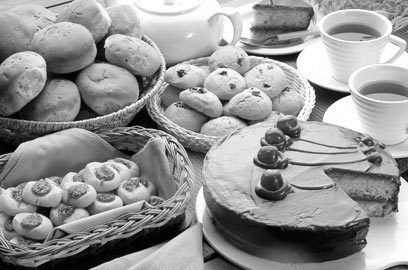
\includegraphics[width=.45\textwidth]{img/barao/padaria.jpg}
\end{figure}

Também são servidos lanches gigantescos, com muitas opções de recheio, por um
preço relativamente barato, então tenha alguém para dividir (acredite, meio
lanche já serve como um almoço completo). Dependendo do recheio, a pizza é muito
barata, também, embora eles não façam entrega. A Alemã fica na Avenida 1. É bom
lembrar que eles servem café da manhã das 7h até às 13h (mas a padaria só fecha
às 22h), então é uma boa pedida para se você não quiser almoçar ou para sábado e
domingo, acordar tarde e tomar um café da manhã para valer pelo almoço.

Na Estrada da Rhodia, próximo à entrada da Cidade Universitária II, há a
Paneteria Di Capri, que tem um pão francês muito bom (a um preço legal) e também
muita variedade (incluindo tortas e lanches). Além disso você também pode tomar
seu café da manhã lá, pois como quase toda padaria eles também oferecem um
cardápio bom para logo cedo. Se você estiver com bastante apetite, de sexta a
domingo eles servem um buffet de café da manhã com muitas opções e a um preço
fixo (em torno de R\$10). Na hora do almoço também são preparados alguns pratos
(para comer no local e para levar) e também há um esquema onde você pede um
grelhado e tem acesso livre a um balcão com saladas e outras coisas, como
petiscos. À noite eles servem pizzas e também há o esquema do grelhado, exceto
no inverno, quando eles servem um buffet de sopas.

Já se você está na Unicamp e quer uma padaria, a dica é a Padaria da FEA (fica
próxima à Cantina da Mecânica). Lá eles têm pães, doces e bolos. Com uma
diferença: há produtos especiais, como pão de queijo com linhaça ou alho e pão
francês com soja. Mas não se assuste: por mais estranho que pareçam, os produtos
de lá são muito bons! E não deixe para ir lá depois das aulas, pois a Padaria da
FEA fecha às 17h.

\subsection{E no fim de semana?}

Nos fins de semana, nem o Bandex nem quase nenhuma cantina da Unicamp abrem (e
as que abrem só o fazem no sábado). Você vai ter que se virar fora da Unicamp.
Na Av. 1 e proximidades tem o Terraço, o Bardana e a Padaria Alemã já citados,
além de vários restaurantes próximos à Alemã. Na Av. 2 tem o Aulus (mais caro no
sábado que durante a semana; domingo, então, mais ainda, mas costuma ter camarão
à milanesa), o Clos Vert (também é caro), um pouco mais pra cima na avenida e,
pouco depois, há o Yaki-Ten, que serve comida chinesa por quilo e japonesa por
pessoa. Logo mais abaixo há o Ilha do Barão. No centro de Barão não faltam
opções. Tem (indo da entrada de Barão pela Estrada da Rhodia) o Estância Grill,
o Barão da Picanha, o Gordão Burguers, o Solar dos Pampas, o Estância
d'Oliveira, o Vila Santo Antonio, o Ki-Pizza, o restaurante Baroneza, o Salsinha
e Cebolinha, o Pão de Açúcar, o McDonald's, o Burger King e vários restaurantes
no Tilli Center (a dica é o Subway, por menos de 10 reais você come bem). Na Av.
Santa Isabel e adjacências tem o Cronópio (numa rua paralela à Santa Isabel), o
Frangonete (próximo ao Santander), o HotDog Central e as Pizzarias Sapore Pizza
e Pizza Fiori. Perto da moradia tem a Tonha (Canto do Acarajé), o Kalunga
Lanches e o famoso dogão da moradia. Por fim, próximo à padaria Di Capri, há
alguns restaurantes mais caros, como a Romana (serviço parecido com o da Di
Capri, porém um bocado mais cara), Pizzaria Gregória, o TBONE (eles também tem
marmitex), o Greg Burgers (o hambúrguer e o milk-shake são excelentes), o Tábua
dos Mares e o Morena-flor.
\begin{figure}[h!]
    \centering
    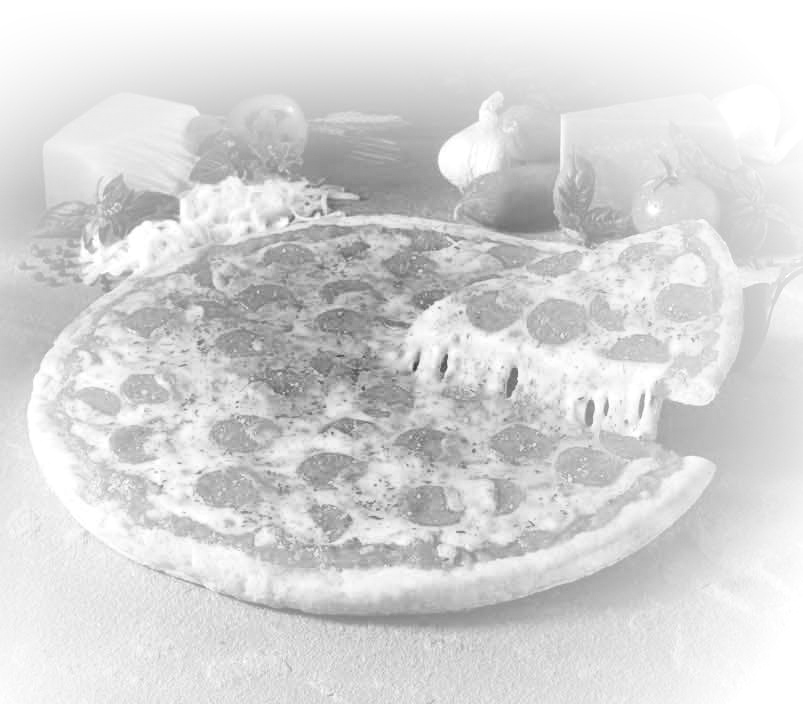
\includegraphics[width=.45\textwidth]{img/barao/pizza.jpg}
\end{figure}


\subsubsection*{Alguns telefones:}

\begin{itemize}
    \item   \textbf{Restaurante Baronesa}
        \\Telefone: (19) 3289-9087
        \\Endereço: Rua Benedito Alves Aranha, 44
        \\Site: \url{restaurantebaronesa.com.br}

    \item   \textbf{China In Box} (Faz entrega em Barão)
        \\Telefone: (19) 3254-5601
        \\Endereço: Rua Romualdo Andreazzi, 333

    \item   \textbf{TBONE Steak Bar}
        \\Telefone: (19) 3289-0485
        \\Endereço: Rua Maria Tereza Dias da Silva, 700

    \item   \textbf{Ginza Bar}
        \\Telefone: (19) 3289-9281
        \\Endereço: Rua Roxo Moreira, 1768

    \item   \textbf{Bardana}
        \\Telefone: (19) 3289-9073
        \\Endereço: Av. Dr. Romeu Tortima, 1500

    \item   \textbf{Terraço}
        \\Telefone: (19) 3289-7920
        \\Endereço: Rua Roxo Moreira, 1344

    \item   \textbf{Pastelaria Oba-Oba}
        \\Telefone: (19) 3249-1908
        \\Endereço: Rua Benedito Alves Aranha, 115

    \item   \textbf{Estância Grill}
        \\Telefone: (19) 3289-6055
        \\Endereço: Av. Albino J. B. de Oliveira, 271
        
    \item   \textbf{Pizza Mais}
        \\Telefone: (19) 3289-0320 / (19) 3289-2754

    \item   \textbf{Barão das Pizzas}
        \\Telefone: (19) 3249-1630
        \\Endereço: Rua Agostinho Pattaro, 187

    \item   \textbf{Pizza Fiori}
        \\Telefone: (19) 3289-3514
        \\Endereço: Av. Santa Isabel, 405

    \item   \textbf{Ki-Pizza}
        \\Telefone: (19) 3289-0863
        \\Endereço: Rua Horácio Leonardi, 76

    % \item   \textbf{Pizza Show}
    %     \\Telefone: (19) 3324-7480

    % \item   \textbf{Terra Nova}
    %     \\Telefone: (19) 3289-4072

    % \item   \textbf{Estação Santa Fe Pizza}
    %     \\Telefone: (19) 3289-4800

    \item   \textbf{Super Mega Pizza}
        \\Endereço: Rua Francisca Resende Merciai, 125B
        \\Telefone: (19) 3288-0606 / (19) 3288-0608
        \\Site: \url{supermegapizza.com}

    \item   \textbf{Vila Ré Pizza}
        \\Telefone: (19) 3289-0321

    \item   \textbf{NADOG'S -- HOT DOG DO NADO}
        \\Telefone: (19) 3029-2270

    \item   \textbf{Casa da Moqueca} (prato mais caro, mas serve duas pessoas)
        \\Telefone: (19) 3289-3131

    \item   \textbf{McDonald's}
        \\Telefone: (19) 3289-0318
        \\Endereço: Av. Albino J. B. de Oliveira, 1430

    \item   \textbf{Subway} (Entrega na região das Av. 1 e 2)
        \\Telefone: (19) 3201-8411 / (19) 3201-8410
        \\Endereço: Av. Albino J. B. de Oliveira, 1556
        \\Site: \url{subdelivery.com.br}
\end{itemize}

\subsection{E à noite?}

\begin{itemize}
    \item   \textbf{Hot-dog Independência:}
        \\Telefone: (19) 3289-8805
        \\Endereço: Rua Angela Signol Grigol, 742
        \\\\
        Tem vários tipos de hot-dogs (com catupiry, com cheddar, com frango
        {\dots}) e tem preços menores que os do Rod Burguers. O único problema é
        que eles cobram taxa de entrega para um lanche e fecham à meia-noite.

    \item   \textbf{Kalunga Lanches:}
        \\Telefone: (19) 3289-5236
        \\Endereço: Rua Sebastião Bonomi, 40
        \\\\
        Perto da moradia, eles não entregam, mas ficam abertos até altas horas.
        Destaque para o caldinho de feijão. Obs: o lugar é limpo e bom.

    \item   \textbf{Mega Sandubão:}
        \\Telefone: (19) 3288-0204
        \\Endereço: Av. Albino J. B. de Oliveira, 2287
        \\\\
        Antigo Ponto Final. Lanchonete localizada na estrada da Rhodia e entrega
        lanches até a meia noite. Muitos gostam bastante dessa lanchonete pela
        famosa maionese temperada que eles servem, não se esqueça de pedir
        quando for comprar lanches.

    \item   \textbf{Barão Hamburgueria:}
        \\Telefone: (19) 3289-9753
        \\Endereço: Av. Albino J. B. de Oliveira, 476
        \\\\
        Rua Localizada na entrada de Barão Geraldo servem lanches parecidos com
        os do Mega Sandubão, lá eles dão outro tipo de maionese e em geral os
        preços são tão caros quanto do Mega Sandubão. Também entregam até meia
        noite.

    \item   \textbf{Lanchão \& Cia:}
        \\Telefone: (19) 3289-3665
        \\Endereço: Av. Albino J. B. de Oliveira, 1214
        \\Site: \url{lanchaoecia.com.br}
        \\\\
        Um dos melhores lanches de Campinas (quiçá o melhor). Os lanches
        geralmente são grandes e muito bons, e os preços são compatíveis com a
        qualidade e quantidade. Eles servem no carro se você preferir, com uma
        bandeja que fica presa no vidro. Fica no centro de Barão Geraldo,
        proximo ao Santander e Pão de Açúcar. Destaque para a batata frita,
        feita de uma forma muito diferente, extremamente crocante e quase
        cremosa por dentro.

    \item   \textbf{Burger King:}
        \\Endereço: Av. Albino J. B. de Oliveira, 1000
        \\\\
        Aberto das 10h às 22h

    \item   \textbf{Ponto 1:}
        \\Telefone: (19) 3289-2378
        \\Endereço: Rua Eduardo Modesto, 54
        \\Site: \url{ponto1bar.com}

    \item   \textbf{Sapore Pizza:}
        \\Telefone: (19) 3289-0228
        \\Endereço: Av. Santa Isabel, 326
        \\\\
        Para quando você estiver com pelo menos mais um amigo para rachar a
        pizza, acaba sendo uma boa pedida. Geralmente as pizzas de mussarela e
        de calabreza estão com preços bem acessíveis. Também entregam até
        meia-noite.

    \item   \textbf{McDonald's:}
        \\Telefone: (19) 3289-5840
        \\Endereço: Av. Albino J. B. de Oliveira, 1430
        \\\\
        Dispensa apresentações. Entregas das 11h às 23h.

    \item   \textbf{Barraquinhas:}
        \\Há várias barraquinhas de hot-dog no centro de Barão e perto da
        moradia. Destaque para o dog do terminal, o Hot Dog Central, o Pedrogue
        e o dogão da moradia. Se você quiser um lanche, uma boa pedida é o Star
        Tresh (Raimundão ou Guarujá, chame como você quiser), que fica perto do
        balão da Avenida 2 e costuma ficar aberto até altas horas. Perto da
        Unicamp, ao lado do posto Ipiranga que fica na avenida 1 também tem um
        dog prensado muito bom e barato.
\end{itemize}

\subsection{Marmitex}

Entrega em casa. Bom e barato.

\begin{itemize}
    \item   \textbf{Tia Rita}
        \\Telefone: (19) 3249-2899

    \item   \textbf{Hailton}
        \\Telefone: (19) 3249-0153
\end{itemize}

Obs: A Sapore Pizza também entrega Marmitex.

\begin{figure}[h!]
    \centering
    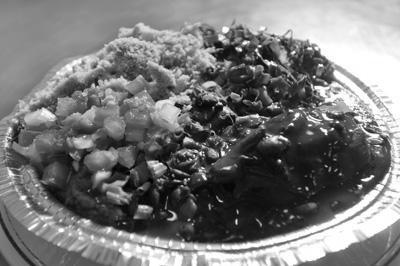
\includegraphics[width=.45\textwidth]{img/barao/marmitex.jpg}
\end{figure}

\subsection{Bares, lanchonetes e restaurantes}

\begin{figure}[h!]
    \centering
    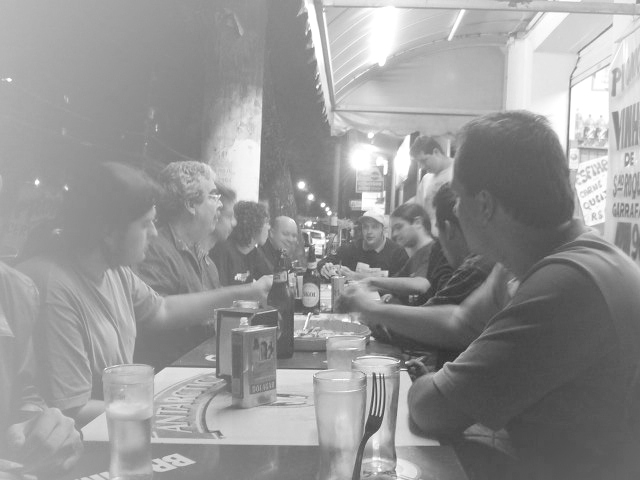
\includegraphics[width=.45\textwidth]{img/barao/bar.jpg}
\end{figure}

\begin{itemize}
    \item   \textbf{Açaizeiro Brasil:} Serve um açaí muito bom e vários tipos de
        comidas mais leves, como lanches naturais, crepes e saladas, além de
        vários sucos. O preço não é caro e a comida é boa.
        \\Endereço: Av. Santa Isabel, 518
        \\Telefone: (19) 3365-6555

    \item   \textbf{Aulus VideoBar \& Restaurant:} A comida é muito boa, porém
        cara, especialmente no final de semana. A exceção fica no preço do
        marmitex, apenas R\$ 10. O ambiente do restaurante é muito diferenciado,
        com bicicletas e ferroramas no teto, por exemplo.
        \\Endereço: Av. Prof. Atílio Martini, 939
        \\Telefone: (19) 3289-4453
        \\Site: \url{aulus.com.br}

    \item   \textbf{Bagdá Café -- Bar \& Esfiharia:} Esfihas boas, mas um pouco
        caras. Entregam em Barão (cardápio no site), mas em horários de pico
        costumam demorar um pouco. A música ambiente inclui música ao vivo e
        ritmos variados, desde a MPB ao Blues.
        \\Endereço: Av. Santa Isabel, 246
        \\Telefone: (19) 3289-0541 / (19) 3289-1842
        \\Site: \url{carlinoamaral.com.br/bagda}

    \item   \textbf{Bar do Coxinha:} Famoso pela coxinha (realmente boa), vale a
        pena ir lá, mas é relativamente caro. Localiza-se perto da avenida Santa
        Isabel, na rua da Sapore Pizza.

    \item   \textbf{Bar do Jair:} Outro lugar famoso pela coxinha: só que esta é
        de carne seca. Fica relativamente perto da Moradia.
        \\Endereço: Rua Eduardo Modesto, 212

    \item   \textbf{Barão da picanha:} Churrascaria rodízio localizada na
        avenida Albino José Barbosa de Oliveira, logo na entrada de Barão.

    \item   \textbf{Batataria Suiça:} Do lado do Mega Sandubão, serve batatas
        recheadas bem diferentes. É um pouco caro, mas vale a pena conferir. Uma
        dica é que às terças-feiras você compra uma batata, mas recebe duas.
        \\Endereço: Estrada da Rhodia -- Praça José Geraldi, a 50m do posto Esso
        \\Telefone: (19) 3201-1174
        \\Site: \url{battataria.com.br}

    \item   \textbf{Boi Falô:} O restaurante é uma rancho, com comida típica do
        interior. É excelente, mas um pouco caro (cerca de R\$30,00 por pessoa),
        um lugar perfeito para levar seus pais quando eles vêm te visitar (e
        pagam o almoço!). Abre apenas nos almoços de sábado e domingo.
        \\Endereço: Rua do Sol, 600
        \\Telefone: (19) 3289-6671 / (19) 3287-6342

    \item   \textbf{Cachaçaria Água Doce:} Localizada na avenida 1, é um lugar
        frequentado por pessoas mais velhas, ótimo para comida e bebida (pinga,
        especialmente), mas é bem caro.

    \item   \textbf{Casa São Jorge:} Música ao vivo todas as noites, com boa
        variedade. Localiza-se na rua Santa Isabel, mais ou menos perto da
        moradia.

    \item   \textbf{Empório Nono:} Caro, tem um chopp muito bem tirado e os
        melhores petiscos de Campinas. Localiza-se na avenida Albino José
        Barbosa de Oliveira, quase em frente ao terminal.

    \item   \textbf{Estância Grill:} Logo na entrada de Barão. Tem rodízios de
        carne e de pizza à noite.
        \\Endereço: Av. Albino J. B. de Oliveira, 271
        \\Telefone: (19) 3289-8697 / (19) 3289-6055 / (19) 3289-1511

    \item   \textbf{Fernando's:} No centro de Barão, perto do Banespa, serve
        cerveja e lanches baratos e muito bons principalmente porque vêm
        acompanhados de uma porção pequena de fritas! Um lugar simples mas muito
        limpo e agradável principalmente em relação ao atendimento. Fecha as 23h
        se segunda a quinta e sábado, tem música ao vivo na sexta e por enquando
        ainda não abre nos domingos.

    \item   \textbf{Fran's Café:} Cafeteria. Vende lanches, cafés, doces,
        salgados e bebidas (quentes ou geladas). Fazem também cafés da manhã.
        Mas é um pouco caro.
        \\Endereço: Av. Albino J. B. de Oliveira, 1600

    \item   \textbf{Greg Burguers:} Uma lanchenete muito boa, mas também muito
        cara.  Uma das especialidades lá é o milk-shake (realmente muito bom).
        Fica na estrada da Rhodia (na esquina da Paneteria Di Capri). Só
        funciona à noite, de terça a domingo.
        \\Endereço: Rua Maria Tereza Dias da Silva, 664
        \\Telefone: (19) 3289-6400
        \\Site: \url{gregburgers.com.br}
\end{itemize}

\begin{figure}[h!]
    \centering
    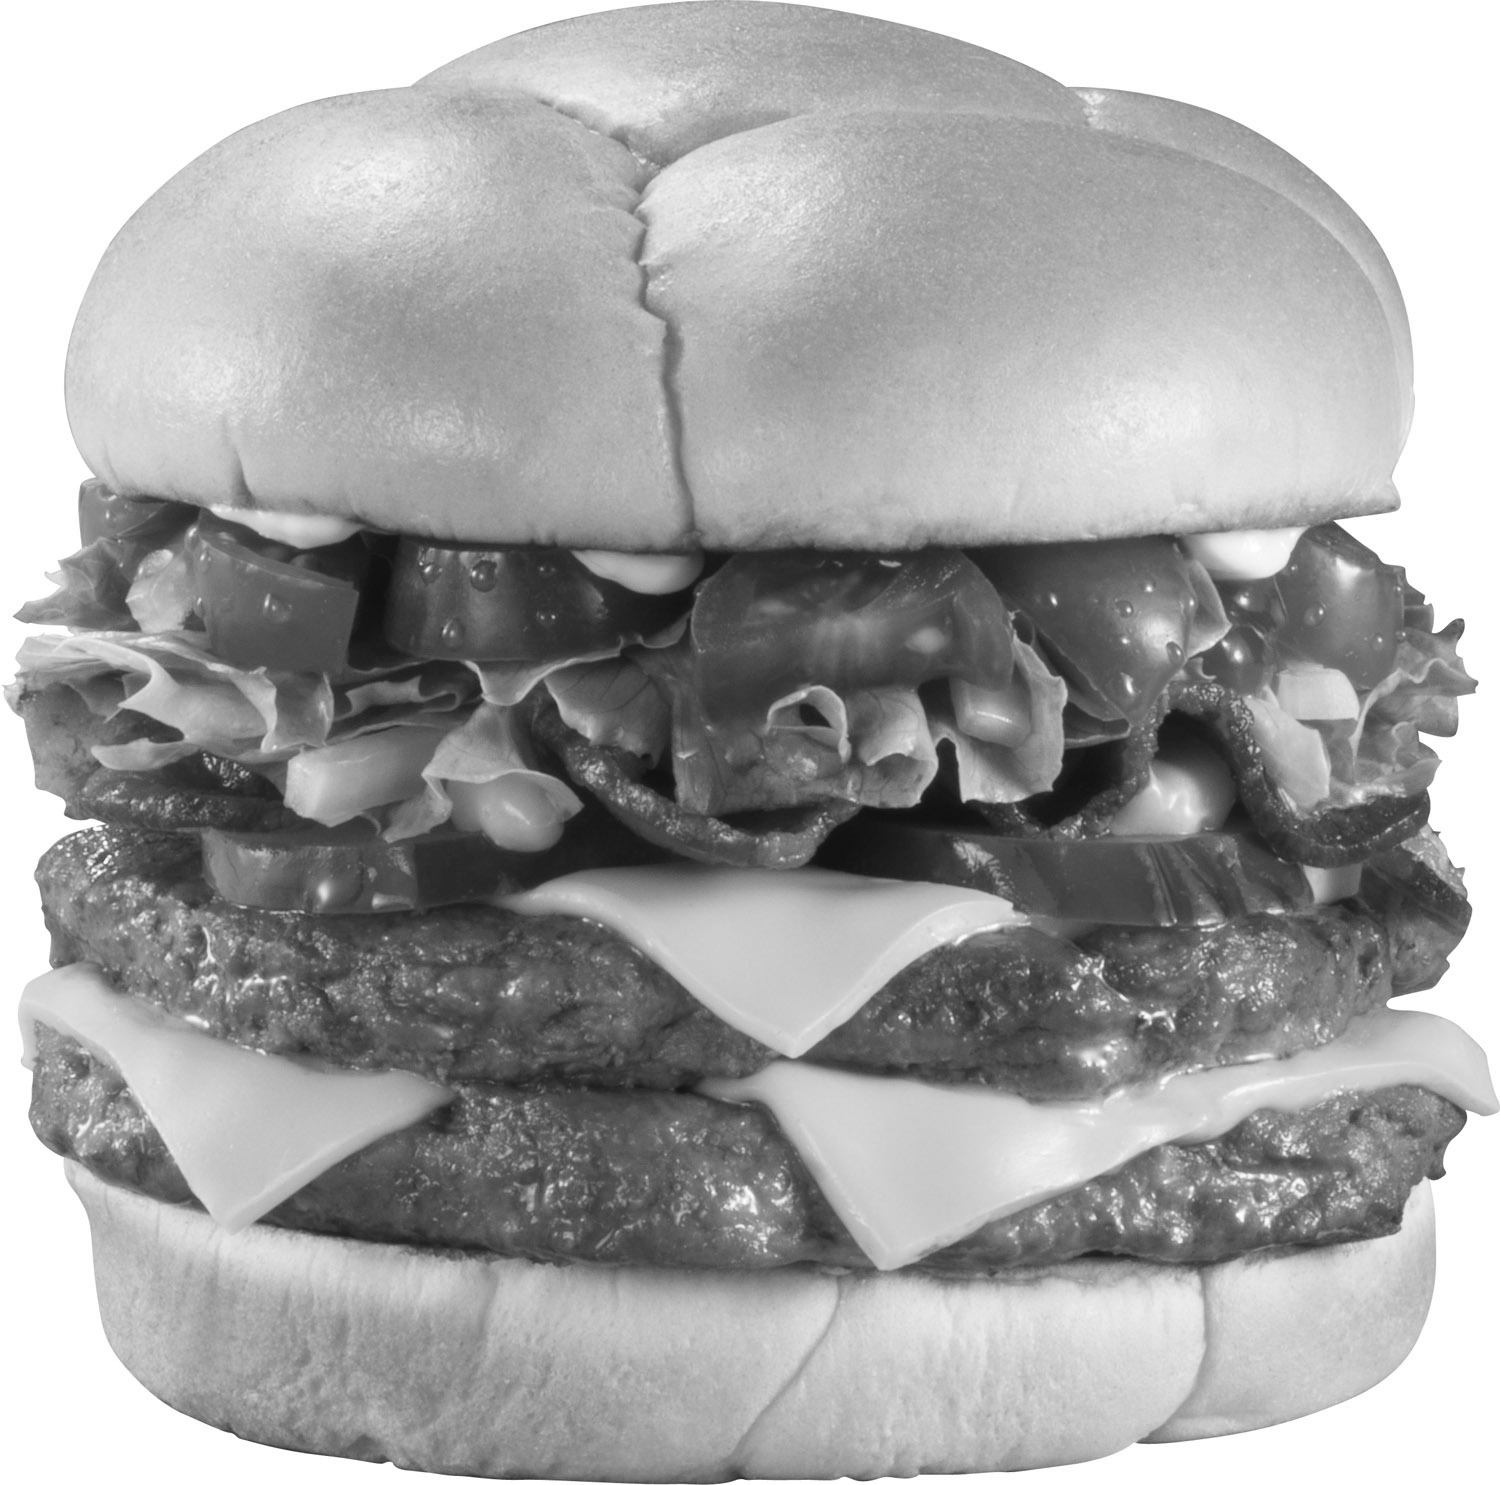
\includegraphics[width=.45\textwidth]{img/barao/burger.jpg}
\end{figure}

\begin{itemize}
    \item   \textbf{La Salamandra:} Restaurante mexicano, localizado ao lado do
        Makis Place. Comida boa e preço compatível, ele tem uma barraquinha na
        feirinha do CB, às quartas.
        \\Endereço: Av. Albino J. B. de Oliveira, 998
        \\Telefone: (19) 3289-2011 / (19) 9277-4340 / (19) 3365-0354

    \item   \textbf{Makis Place:} Temakeria próxima ao terminal.
        \\Endereço: Av. Albino J. B. de Oliveira, 976
        \\Telefone: (19) 3367-3077
        \\Site: \url{makis.com.br}

    \item   \textbf{Mega Sandubão:} Já comentado acima, fica aberto até altas
        horas.  Mas à noite serve cerveja também a um bom preço. Localiza-se na
        estrada da Rhodia (continuação da avenida Albino José de Oliveira).
        \\Endereço: Av. Albino J. B. de Oliveira, 2287
        \\Telefone: (19) 3288-0204

    \item   \textbf{Quintal do Neto:} No alto da avenida 1, perto do balão de
        entrada em Barão Geraldo, tem cerveja a preços razoáveis, salgados
        (coxinha e quibe) grandes, e mesas de sinuca (de ficha e por hora).

    \item   \textbf{Rudá:} Localizado na Santa Isabel, bar com música ambiente.

    \item   \textbf{Solar dos Pampas:} Buffet excelente. Custa R\$ 24,00 apenas
        a comida e R\$ 34,00 com refrigerante e suco incluídos (o tanto que você
        conseguir beber). Fazem um esquema no aniversário das pessoas que sai
        por R\$ 18,00 com rodízio, cerveja, refrigerante, buffet, sorvete e
        pinga à vontade. Ao lado do Estância d'Oliveira.
        \\Endereço: Av. Dr. Romeu Tortima, 165
        \\Telefone: (19) 3289-1484 / (19) 3289-7869

    \item   \textbf{Star Clean:} É o bar mais próximo à Unicamp, e por isso está
        sempre cheio. Principal ponto de encontro depois da aula e tem um bom
        preço.

    \item   \textbf{Subway:} Lanchonete. Vende dos mais variados tipos de
        lanches.  Lanches muito bons, e não tão caros. Localiza-se no Tilli
        Center (avenida Albino José Barbosa de Oliveira, 1556, esquina com a
        avenida 2). Do lado do Subway tem um caixa 24 horas que trabalha com os
        principais bancos. O Subway faz entregas em algumas regiões de Barão.
        \\Site: \url{subdelivery.com.br}

    \item   \textbf{Temakeria:} Lugar relativamente novo, meio caro. Vende só
        temaki e bebidas. O horário de funcionamento é bastante conveniente.
        \\Endereço: Av. Dr. Romeu Tortima, 1259
        \\Telefone: (19) 3289-0802
        \\Horário de funcionamento: domingo a terça das 11h30 às 0h, quarta a
        sábado das 11h30 às 6h
        \\Site: \url{tmkr.com.br}

    \item   \textbf{Estância d'Oliveira:} Antigo Universo das Massas. Rodízio de
        massas perto do Terminal. Bom e não é caro. De domingo à noite é o
        horário mais barato e dá pra encher bem o bucho de massa. Depois de ir
        até lá, você não vai querer saber de comer massas por um bom tempo.
        \\Endereço: Av. Albino J. B. de Oliveira, 576
        \\Telefone: (19) 3289-5369

    \item   \textbf{Vila Ré -- Pizza:} Pizzaria próxima do terminal e do
        supermercado Dalben. Tem alguns sabores diferentes, as pizzas são boas e
        o preço não é alto. Possui serviço de entrega das 18h às 23h.
        \\Endereço: Av. Albino J. B. de Oliveira, 658
        \\Telefone: (19) 3289-0319

    \item   \textbf{Bar do Zé:} O pub tem apresentações ao vivo todas as
        semanas.  Localiza-se também na avenida Albino José de Oliveira, bem em
        frente ao Pão de Açúcar.
        \\Site: \url{obardoze.com.br}

    \item   \textbf{Echos Studio Bar:} Um bar relativamente novo, possui
        apresentaçes ao vivo direto, que costumam ser de Rock, Blues ou Jazz.
        Fica entre a Santa Isabel e Albino J. B. de Oliveira.
        \\Endereço: Rua Agostinha Pátaro, 54
        \\Site: \url{echo.mus.br}

    \item   \textbf{Marambar:} Possui bebidas, lanches, sucos e porções a preços
        razoáveis. Ambiente agradável, ao ar livre, muito próximo da Unicamp.
        Bastante frequentado por computeiros e engenheiros em geral, além de
        muita gente de outros cursos. Funciona de segunda a sexta, das 7h30 até
        as 2h30, e aos sábados, das 9h até a 1h.
        \\Endereço: Av. Dr. Romeu Tortima, 1538 (próximo ao balão da avenida 1)
        % \\Telefone: (19) 3289-0080
\end{itemize}
